\chapter{Molecular modeling of biological membranes}

  Intro.

\section{Classical molecular dynamics simulations}

\section{Including polarizability}

  Lit. research on how people include polarizability in classical simulations. 

\subsection{Electronic continuum correction as implicit treatment of electronic polarizability}

  Tell what it is.

\section{Including polarizability in classical MD models of lipids through ECC}

  Tell what I did.
  -- ECC-POPC paper and ongoing research with DPPC, POPE and POPS.
  ECC-Charmm36 ? (very marginally)

\subsection{Structural parameters of a pure ECC-POPC model membrane: Agreement with experiments} 
 
\begin{figure}[tb!] 
  \centering 
  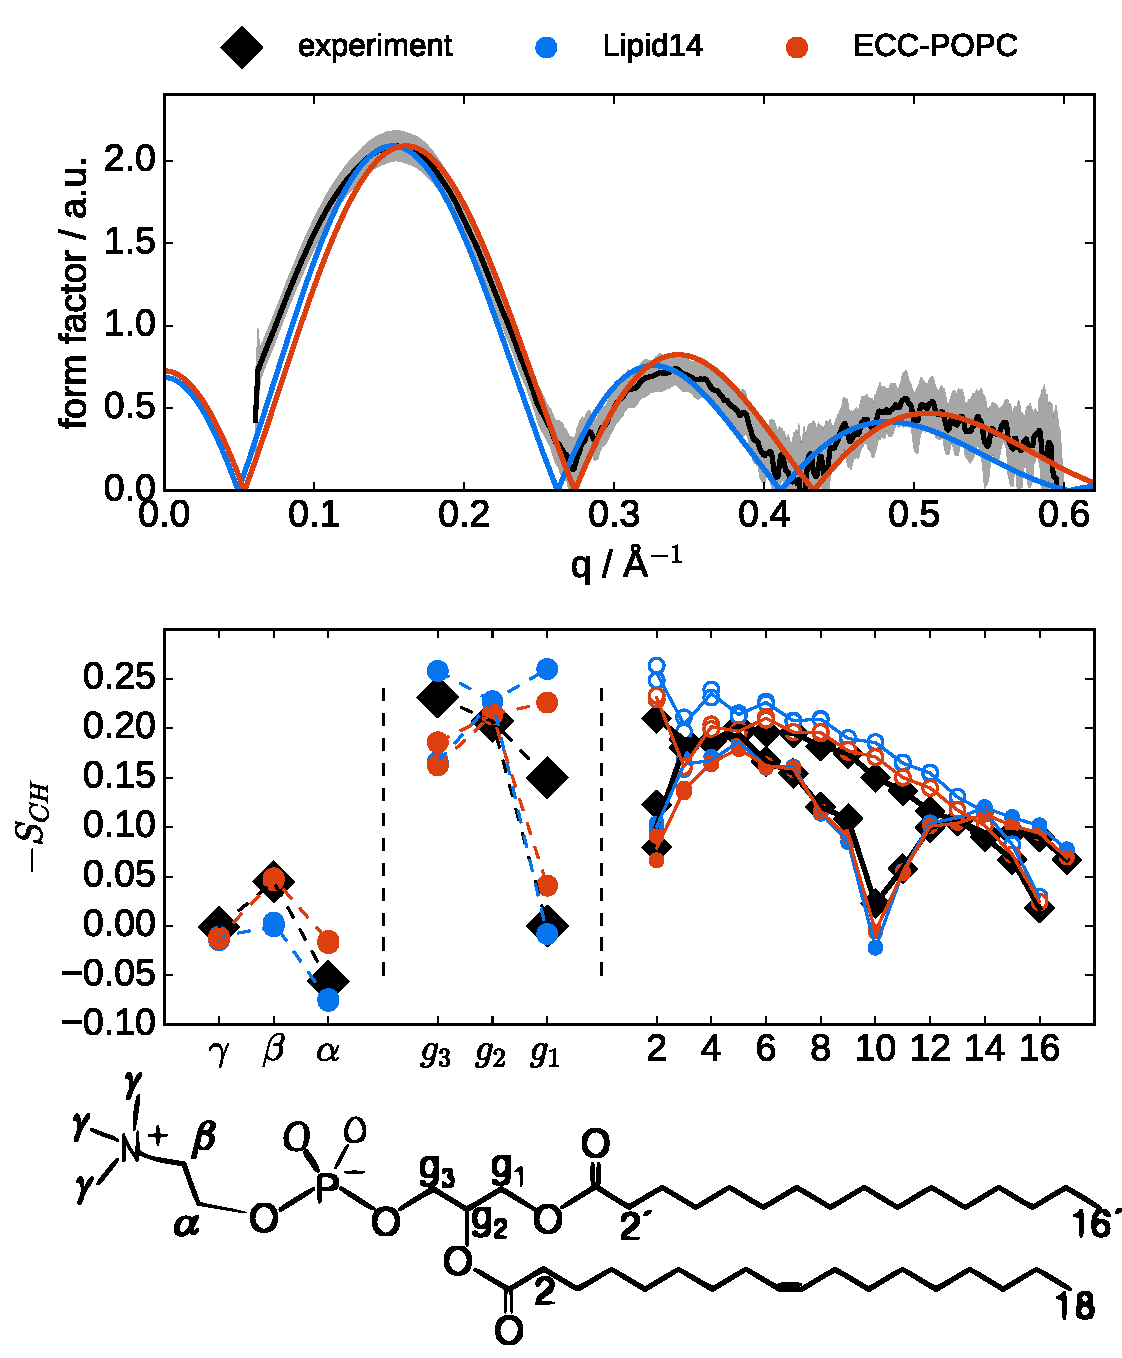
\includegraphics[width=8.2cm]{../img/ecc_pops/Order-parameters_form-factors_exp-L14-ECCL17_q80_sig89_POPC-struct.pdf} 
  \caption{ \label{simVSexpNOions} 
    Top: X-ray scattering form factors from simulations with the Lipid14 \cite{dickson14} and 
    the ECC-POPC models compared with experiments~\cite{kucerka11} at 303~K. \\
    Middle: Order parameters of POPC head group, glycerol backbone and acyl chains  
    from simulations with the Lipid14 \cite{dickson14} and the ECC-POPC models 
    compared with experiments \cite{ferreira13} at 300~K. 
    The size of the markers for the head group order parameters correspond to 
    the error estimate $\pm 0.02$ for experiments \cite{botan15,ollila16}, 
    while the error estimate for simulations is $\pm 0.005$
    (Bayesian estimate of 95\% confidence interval \cite{scipy}).
    The size of the points for acyl chains are decreased by a factor of 3 to improve the clarity of the plot.
    Open/closed symbols are used for palmitoyl/oleoyl chains of POPC. \\
    Bottom: The chemical structure of POPC and the labeling of the carbon segments. 
  }  
\end{figure} 
 
\begin{table}[tb!] 
  \caption{Values of the area per lipid (APL) of POPC bilayers without ions. \label{tab:apls} 
  } 
  \begin{tabular}{l|c c} 
    model          & APL (Å$^2$)   & Temperature [K] \\ 
    \hline 
    Lipid14                   & 65.1$\pm$ 0.6  &  300 \\ 
    Lipid14 \cite{dickson14}  & 65.6$\pm$ 0.5  &  303 \\ 
    \hline 
    ECC-POPC                & 63.2$\pm$ 0.6  &  300       \\ 
    \hline 
    experiment \cite{kucerka11} & 64.3  &  303    \\ 
    \hline 
  \end{tabular} 
\end{table} 
 
 
First, we present results for bilayers in pure water. 
The ECC-POPC and Lipid14 models both reproduce the experimental X-ray scattering form factors 
of a POPC bilayer with a comparable accuracy (see Fig.~\ref{simVSexpNOions}). 
The area per lipid from the Lipid14 model is by $\approx$1Å larger than the 
experimental value in Table~\ref{tab:apls}, while the value from the ECC-POPC model 
is by $\approx$1Å smaller than the experimental one. 
The values of the area per lipid of the ECC-POPC model vary slightly 
when simulated with different water models (i.e., within the interval of 62.2--66.8 Å, see Table~S2 in SI), 
while still being close to the experimentally reported values. 
We can thus conclude that the ECC-POPC model reproduces the experimental dimensions of the POPC 
lipid bilayer with a comparable accuracy to other state-of-the-art lipid models~\cite{ollila16}. 
 
 
Similarly, the acyl chain order parameters of the ECC-POPC model, as well as those of the Lipid14 model~\cite{dickson14}, agree with the experimental values within the error bars, as presented in Fig.~\ref{simVSexpNOions}. Notably, the experimentally measured forking and small order parameter values of the $C_2$ segment in {\it sn}-2 chain are well reproduced by both models. This feature has been suggested to indicate that the carbonyl of the {\it sn}-2 chain is directed towards the water phase, in contrast to the carbonyl in the {\it sn}-1 chain, which orients more along the bilayer plane~\cite{seelig75,schindler75,gawrisch92}. 
This arrangement, which is not fully reproduced by other available lipid models~\cite{ollila16}, may be a relevant feature for the ion binding details. 
 
The order parameters of the $\alpha$ and $\beta$ carbons in the head group are slightly larger in the ECC-POPC model than in the Lipid14 model, which is apparently related to the P-N vector orienting by about 7$^{\circ}$ more toward the water phase in the former model, see Fig.~\ref{OrderParameterCHANGESsurf}. While both models perform relatively well, considering the available experimental evidence, it is not possible to decide which of the two models provides more realistic head group orientations. The ECC-POPC model gives the $\beta$ carbon order parameter value closer to experiments than the Lipid14 model, while the opposite is true for the $\alpha$ carbon. The accuracy of both models in the glycerol backbone region is comparable to other state-of-the-art lipid model available in literature \cite{botan15}, see Fig.~\ref{simVSexpNOions}. 

\subsection{Calibration of head group response to membrane-bound charge using cationic surfactant}\label{section:boundCHARGE} 
 
\begin{figure}[tb!] 
  \centering 
  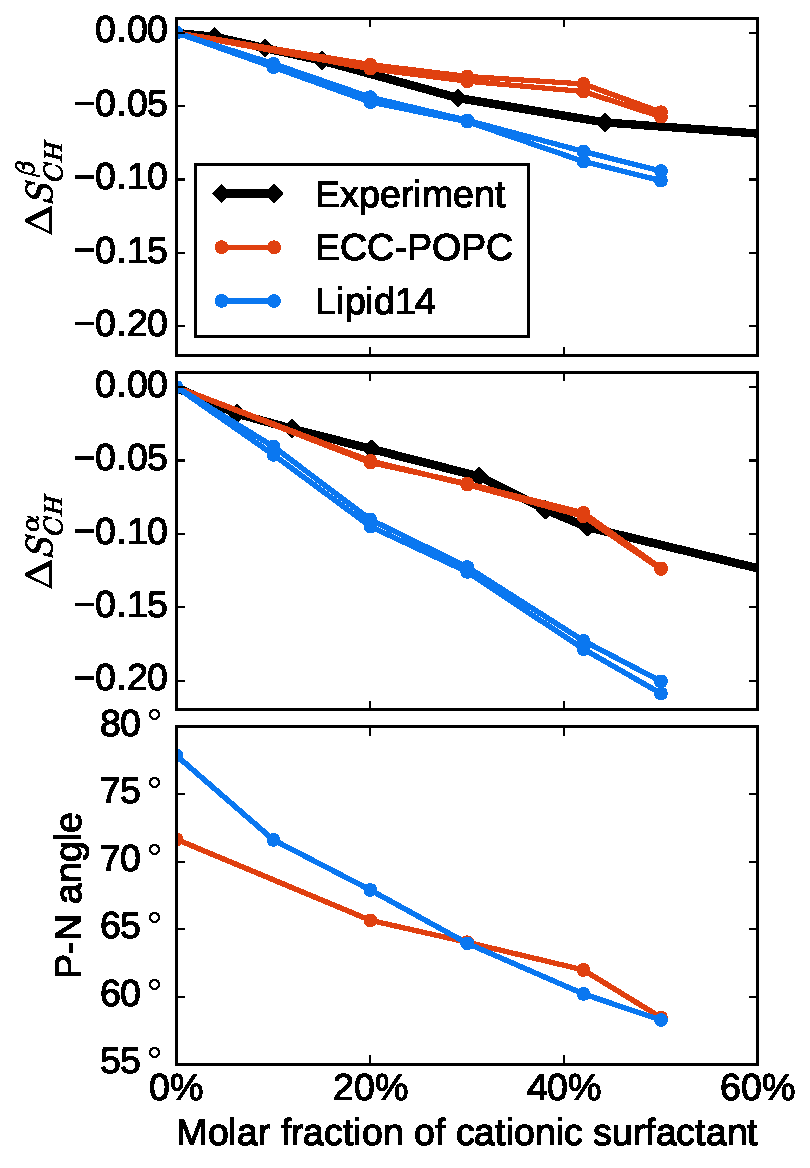
\includegraphics[width=8.0cm]{../img/ecc_pops/PN_angle_OrdPars-A-B_L14-ECCL17_q80_sig89_surf.pdf} 
  \caption{\label{OrderParameterCHANGESsurf} 
    The changes of head group order parameters and P-N vector orientation as a function of 
    a molar fraction of the cationic surfactant dihexadecyldimethylammonium in a POPC bilayer 
    from simulations and experiments \cite{scherer89} at 313 K.
  } 
\end{figure} 
 
Before studying the sodium and calcium ion binding affinities, we quantify the response of the head group order parameters to the amount of bound charge by using mixtures of monovalent cationic surfactants (dihexadecyldimethylammonium) and POPC~\cite{scherer89}. These mixtures have a well-defined amount of bound charge per PC, namely, the molar fraction of cationic surfactants. This is due to the ability of dihexadecyldimethylammonium to directly insert in the lipid bilayer due to its two hydrophobic acyl chains. Furthermore, available experimental data for these systems can be used to validate the sensitivity of lipid head group order parameters to the amount of bound charge in simulations \cite{scherer89}. 
 
The changes of the head group order parameters with increasing amount of the cationic surfactant are compared between simulations and experiments~\cite{scherer89} in Fig.~\ref{OrderParameterCHANGESsurf}. An approximately linear decrease of the order parameters, as expected from Eq. \ref{OPchangeEQ}, is observed in both simulations and experiments at least for mole fractions below $\sim$30\%. The slope is, however, too steep in the Lipid14 model indicating that the response of head group order parameters to the bound positive charge is too strong. In contrast, the slope of the ECC-POPC model is in a very good agreement with experiments for the $\alpha$ segment, while being only slightly underestimated for the $\beta$ segment. 
 
In Fig.~\ref{OrderParameterCHANGESsurf}, we show the headgroup P-N vector angle as a function of the mole fraction of the cationic surfactant. As suggested previously~\cite{seelig87}, the headgroup orients more towards the water phase with the increasing amount of positive charge in the PC lipid bilayer. The effect is more pronounced in the Lipid14 model than in the ECC-POPC model.   For example, the addition of 50\% mole fraction of the cationic surfactant leads to a decrease of 20$^{\circ}$ of the P-N vector angle for the Lipid14 model while only of 11$^{\circ}$ in the ECC-POPC model. The difference is in line with the smaller order parameter changes and the reduced charge--dipole interactions in the latter model. The weaker sensitivity of the P-N vector angle response in the ECC-POPC model is in better agreement with experiments. 
 
 
\subsection{Validation of ECC-POPC model using binding affinities to Na$^+$ and Ca$^{2+}$ cations: the electrometer concept} 
 
 
\begin{figure}[htb!] 
  \centering 
  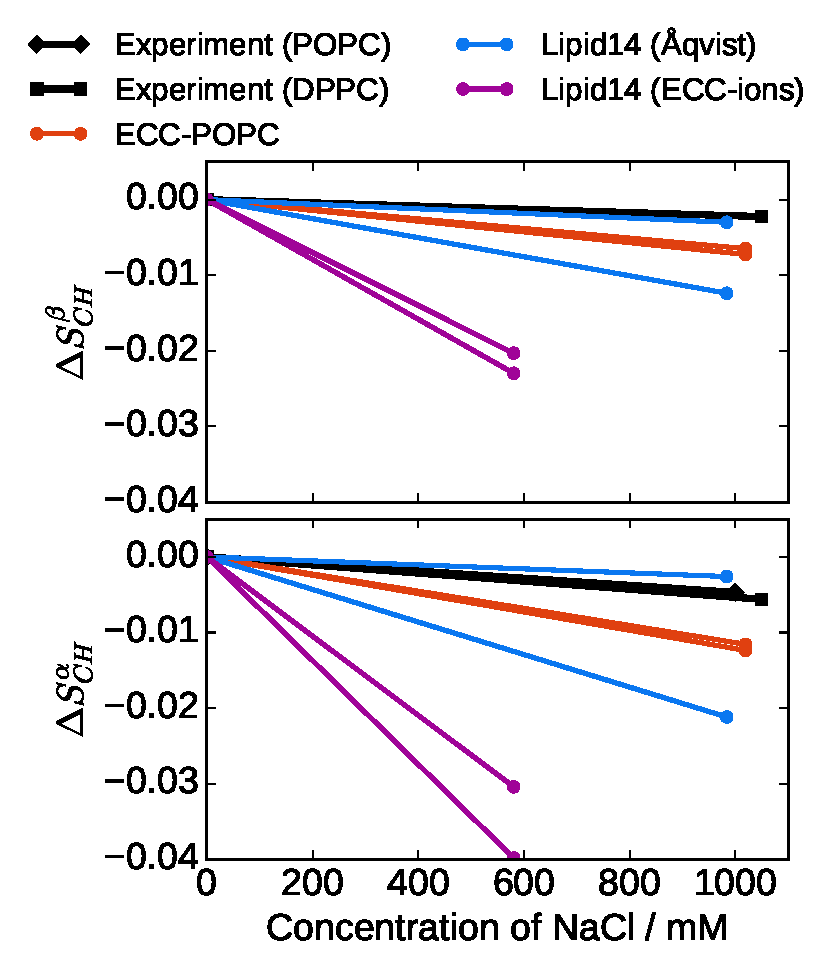
\includegraphics[width=8.0cm]{../img/ecc_pops/OrdPars-A-B_L14-ECCL17_q80_sig89_NaCl.pdf} 
  \caption{\label{fig:delta_ordPar_NaCl} 
    Changes of the head group order parameters of a POPC bilayer as a function of NaCl concentration 
    in bulk ($C_{ion}$) from simulations with different force fields at 313 K together with  
    experimental data for DPPC (323\,K) \cite{akutsu81} and POPC (313\,K) \cite{altenbach84}. 
    Simulation data with Lipid14 and Åqvist ion parameters at 298 K are taken directly from 
    Refs.~\cite{lipid14POPC0mMNaClfiles,lipid14POPC1000mMNaClfiles}. 
  } 
\end{figure} 
 
\begin{figure}[htb!] 
  \centering 
  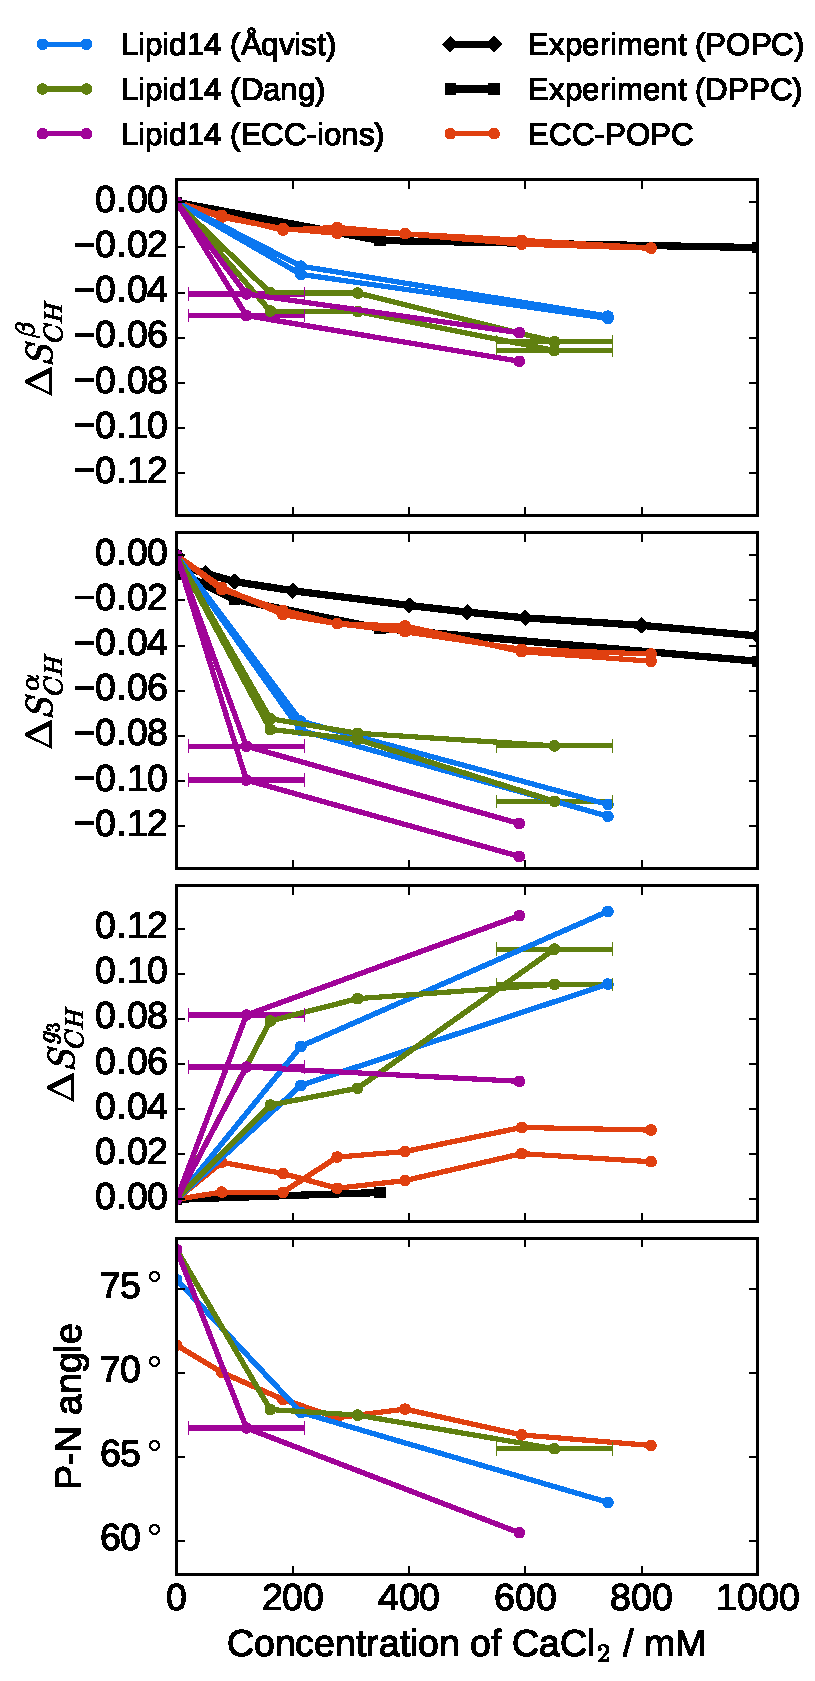
\includegraphics[width=8.0cm]{../img/ecc_pops/PN_angle_OrdPars-A-B-g3_L14-ECCL17_q80_sig89_CaCl.pdf} 
  \caption{\label{fig:delta_ordPar_CaCl} 
    Changes of the head group order parameters and P-N vector orientation of a POPC bilayer  
    as a function of the CaCl$_2$ concentration in bulk ($C_{ion}$) 
    from simulations at 313 K together with experimental data  
    (DPPC (323\,K) \cite{akutsu81} and POPC (313\,K) \cite{altenbach84}).  
    The error estimate for bulk concentrations is approximately 10\,mM. 
    The order of magnitude larger error in the
    simulation with Lipid14 and ECC-ions is due to unconverged bulk densities  (shown if Fig.~\ref{fig:cacl-dens}) limited by
    the simulation box.  
    Simulation data with Lipid14 and Åqvist ion parameters at 298 K are taken directly from 
    Refs.~\citenum{lipid14POPC0mMNaClfiles,lipid14POPC350mMCaClfiles,lipid14POPC350mMCaClfilesNC}. 
  } 
\end{figure} 
 
Changes of the lipid bilayer head group order parameters extracted from simulations and 
experiments \cite{akutsu81, altenbach84} are shown in Figs.~\ref{fig:delta_ordPar_NaCl} 
and~\ref{fig:delta_ordPar_CaCl} as functions of NaCl or CaCl$_2$ concentrations. 
As seen in Fig.~\ref{OrderParameterCHANGESsurf}, the order parameters decrease 
proportionally to the amount of the bound positive charge. 
These results can be thus used to compare the ion binding affinities to lipid bilayers between 
simulations and experiments using the electrometer concept~\cite{seelig87, catte16}. 
 
The experimentally measured small order parameter 
changes with NaCl (Fig.~\ref{fig:delta_ordPar_NaCl})  
are reproduced by the Lipid14 model simulated with Åqvist ions. 
However, the same combination of models overestimates the order parameter changes with CaCl$_2$ (Fig.~\ref{fig:delta_ordPar_CaCl}). 
Replacing Åqvist ions with ion parameters by Dang et al.~\cite{smith94, chang1999, dang2006} 
or ECC-ions~\cite{martinek17, kohagen16, Pluharova2014} did not improve 
the results~(Figs.~\ref{fig:delta_ordPar_NaCl} and \ref{fig:delta_ordPar_CaCl}). 
In line with the previous work \cite{catte16}, the results suggest that improvements 
in the lipid parameters are required to correctly describe the binding of cations to phospholipid bilayers. 
 
The results from simulations combining the ECC-POPC with the ECC-ion models \cite{martinek17, kohagen16, Pluharova2014} exhibit a significantly improved behavior of the POPC head group order parameters as a function of NaCl or CaCl$_2$ concentrations, see Fig.~\ref{fig:delta_ordPar_NaCl} and Fig.~\ref{fig:delta_ordPar_CaCl}. Considering that we are also able to reproduce the experimental response in systems with known charge density (see above section \ref{section:boundCHARGE}), we conclude that our ECC model correctly reproduces the binding affinities of Na$^{+}$ and Ca$^{2+}$ ions to the POPC lipid bilayer. Furthermore, while the response of the glycerol backbone $g_3$ order parameter to CaCl$_2$ was significantly overestimated in the original Lipid14 model, the ECC-POPC model provides an improved agreement with experiment, as seen in Fig.~\ref{fig:delta_ordPar_CaCl}. 
Also the changes of the P-N vector angle are too pronounced for the Lipid14 model, 
for which the largest tilting toward water phase induced by a $780\,\mathrm{mM}$ 
CaCl$_2$ concentration is approximately 17$^{\circ}$. The corresponding value 
for the ECC-POPC simulation is only 6$^{\circ}$ ($820\,\mathrm{mM}$ CaCl$_2$).  
 
Within the Lipid14 model, the overestimated changes in the lipid headgroup order parameter of POPC  as functions of the CaCl$_2$ concentration arise both from the overestimated binding affinity and the excessive sensitivity of the headgroup tilt to the bound positive charge. It is plausible to assume that the same applies to the other lipid models tested in a previous study~\cite{catte16}, which underlines the importance of validation of the lipid headgroup order parameter response to the bound charge.  
 
Finally, the ion binding affinities for the ECC-POPC model with different water models are compared in SI. In general, the performance of ECC-POPC with any of the tested water models is better than that of the original Lipid14 model, with the order parameter changes being slightly overestimated with the four-site water models and with TIP3P model. 
 
 

\section{How neutral and negatively charged phospholipid membranes interact with ions}

  Results.
  And comments on the published papers. 

  TODO: Dissect the following paragraphs taken from \citenum{melcr18}.

\subsection{Binding affinities of Na$^+$ and Ca$^{2+}$ cations to the POPC membrane} 
\label{sec:affinity} 
 
\begin{table}[tb!] 
  \caption{Bulk concentrations of Ca$^{2+}$ (C$_b$), relative surface excess of calcium with respect to water ($\Gamma_{Ca}^{\rm water}$), 
    and the percetages of Ca$^{2+}$ bound to phosphate or carbonyl oxyges ($r^\mathrm{Ca^{2+}} _\mathrm{PO_4} $ and $r^\mathrm{Ca^{2+}} _\mathrm{O_{carb.}}$) 
    in different POPC bilayer models. All systems have the same molar concentration of Ca$^{2+}$ with respect to water ($C_{ion}'$=350mM). 
  \label{tab:binding}} 
  \begin{tabular}{l|c c | c | c c} 
    model                  & $C_{ion}'$ & $C_{ion}\,/\,\mathrm{mM}$ & $\Gamma_{Ca}^{\rm water} \,/\, \mathrm{nm}^{-2}$  & $r^\mathrm{Ca^{2+}} _\mathrm{PO_4} $ & $r^\mathrm{Ca^{2+}} _\mathrm{O_{carb.}} $ \\ 
    \hline 
    ECC-POPC             &  350  &  $280\pm 10 $  &  $0.06 \pm 0.01 $                           &  99\%  &    25\%    \\ 
    Lipid14/Åqvist     &  350  &  $210\pm 10 $  &  $0.13 \pm 0.01 $                          & 100\%  &    37\%     \\ 
    Lipid14/Dang           &  350  &  $160\pm 10 $  &  $0.23 \pm 0.03 $                            & 100\%  &    14\%    \\ 
    Lipid14/ECC-ions       &  350  &  $120\pm 100$  &  $0.35 \pm 0.11 $                         & 100\%  &    23\%    \\ 
  \end{tabular} 
\end{table} 
 
Binding affinities of Ca$^{2+}$ ions to a POPC bilayer in different simulation models were quantified by calculating the relative surface excess of calcium with respect to water molecules, $\Gamma_{\rm ion}^{\rm water}$, from Eq.~\ref{surfexcess}. 
The values of $\Gamma_{\rm ion}^{\rm water}$ 
from different simulations with the same molar concetration of cations with respect 
to water ($C_{ion}'$=350mM) are shown in Table~\ref{tab:binding}. 
As expected from the changes of the lipid headgroup order parameters in Fig.~ \ref{fig:delta_ordPar_CaCl}, the relative surface excess of calcium, $\Gamma_{\rm Ca}^{\rm water}$ = 0.06~nm$^{-2}$, is significantly smaller for the ECC-POPC model than for the other models, 0.13--0.35~nm$^{-2}$. 
Interestingly, the calculated relative surface excess of \ce{NaCl} at $1\,\mathrm{M}$ concentration (ECC-ions~\cite{Pluharova2014}) using our ECC-POPC model is not only quantitatively but also qualitatively different from \ce{CaCl2} having actually a negative value of $\Gamma_{Na}^{water} = -0.11 \pm 0.01) \rm{nm}^{-2}$ (Fig.~\ref{fig:cacl-dens}. This  
means that on average water molecules are preferred to sodium and chloride ions at the membrane-water interface.   
This is in contradiction with most of the available lipid force fields, which predict a positive surface excess of sodium at PC lipid bilayers \cite{catte16}. 
 
\begin{figure}[htbp!] 
  \centering 
  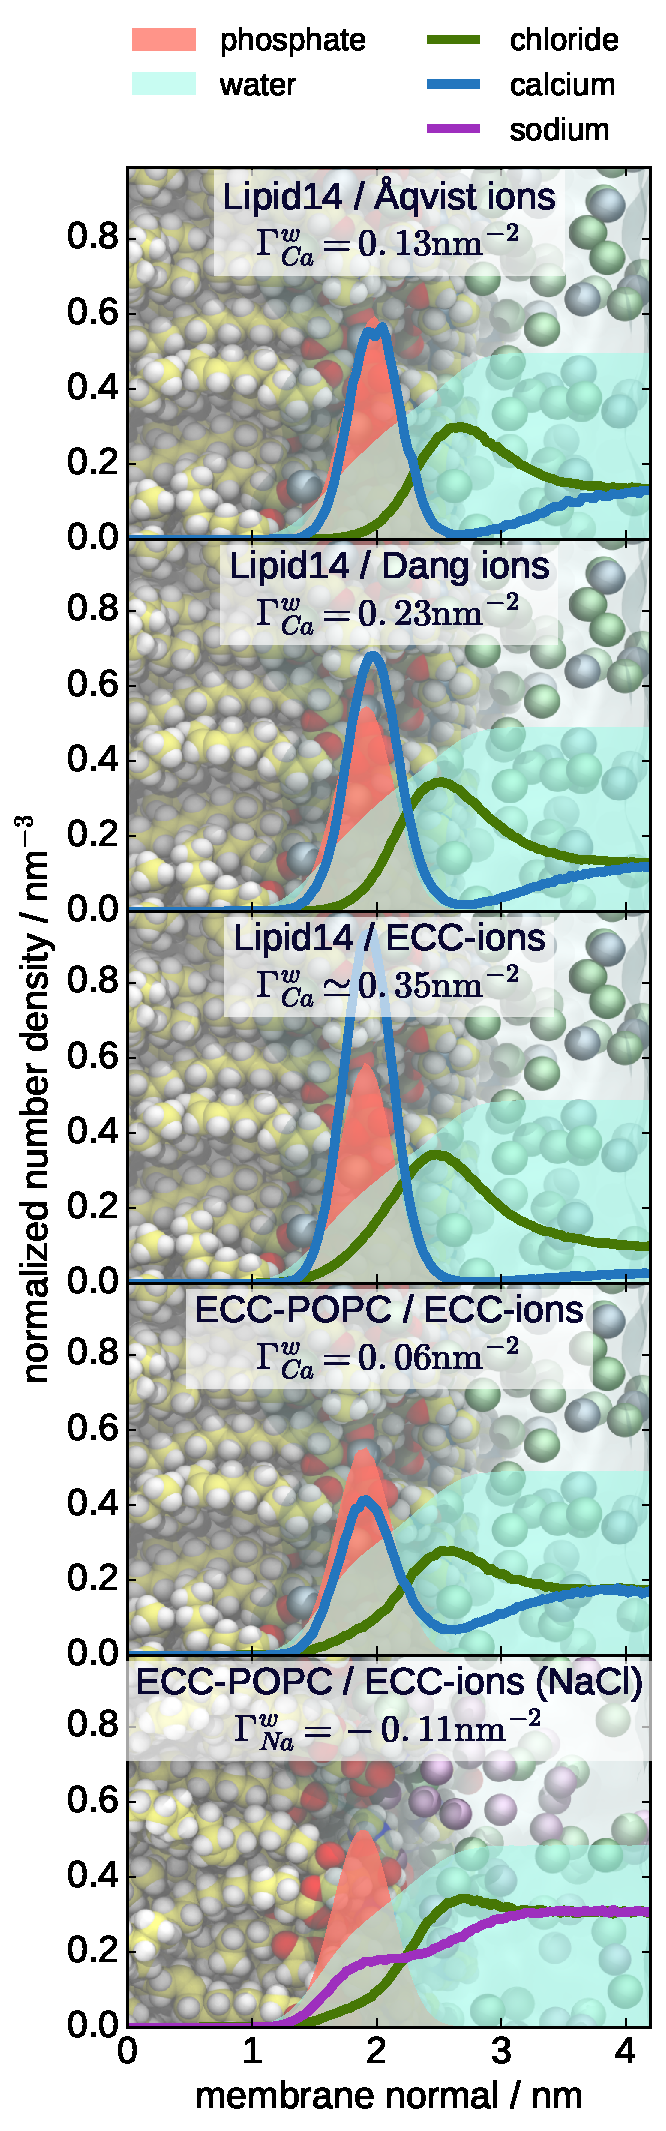
\includegraphics[height=19.9cm]{../img/ecc_pops/density_profiles_ca_cl_wat_phos_models-compar.pdf} 
  \caption{\label{fig:cacl-dens} 
    Number density profiles of \ce{Ca^{2+}}, \ce{Na^{+}} and \ce{Cl^-} along membrane normal axis 
    for different force fields. 
    In order to visualize the density profiles with a scale comparable to the profile of \ce{Ca^{2+}},  
    the density profiles of~\ce{Cl^-} and \ce{Na^{+}} ions are divided by 2, and 
    the density profiles of phosphate groups and water are divided by 5 and 200, respectively.  
    All simulations with \ce{CaCl2} shown here have the same molar concentration of ions in water ($C_{ion}'$=350~mM). 
    The simulation with \ce{NaCl} has $C_{ion}'$=1000~mM. 
    } 
\end{figure} 
 
\subsection{Molecular interactions between Na$^+$ or Ca$^{2+}$ cations and POPC oxygens} 
We analyzed the ratio of the number of calcium cations bound to either phosphate or carbonyl moieties and the total number of bound cations in our POPC bilayers as done previously in Ref.~\citenum{javanainen17}. A maximum distance of 0.3~nm from any lipid oxygen is used to define a bound calcium. The results from ECC-POPC simulation in Table~\ref{tab:binding} show that almost all (99\%) of the bound Ca$^{2+}$ ions are in direct contact with phosphate oxygens. From these ions, only one third (32\%) also interacts with the carbonyl oxygens, while the interaction of calcium ions with carbonyl oxygens only is rare (1\%). The most abundand interaction scenarios between Ca$^{2+}$ ions and phosphate oxygens are visualized using the probability density isocontours in Fig.~\ref{fig:volmaps}. While higher concentrations of \ce{CaCl2} increase the number of contacts per lipid, the distribution of contacts between phosphate and carbonyl oxygens is not affected. 
 
\begin{figure}[tb!] 
  \centering 
  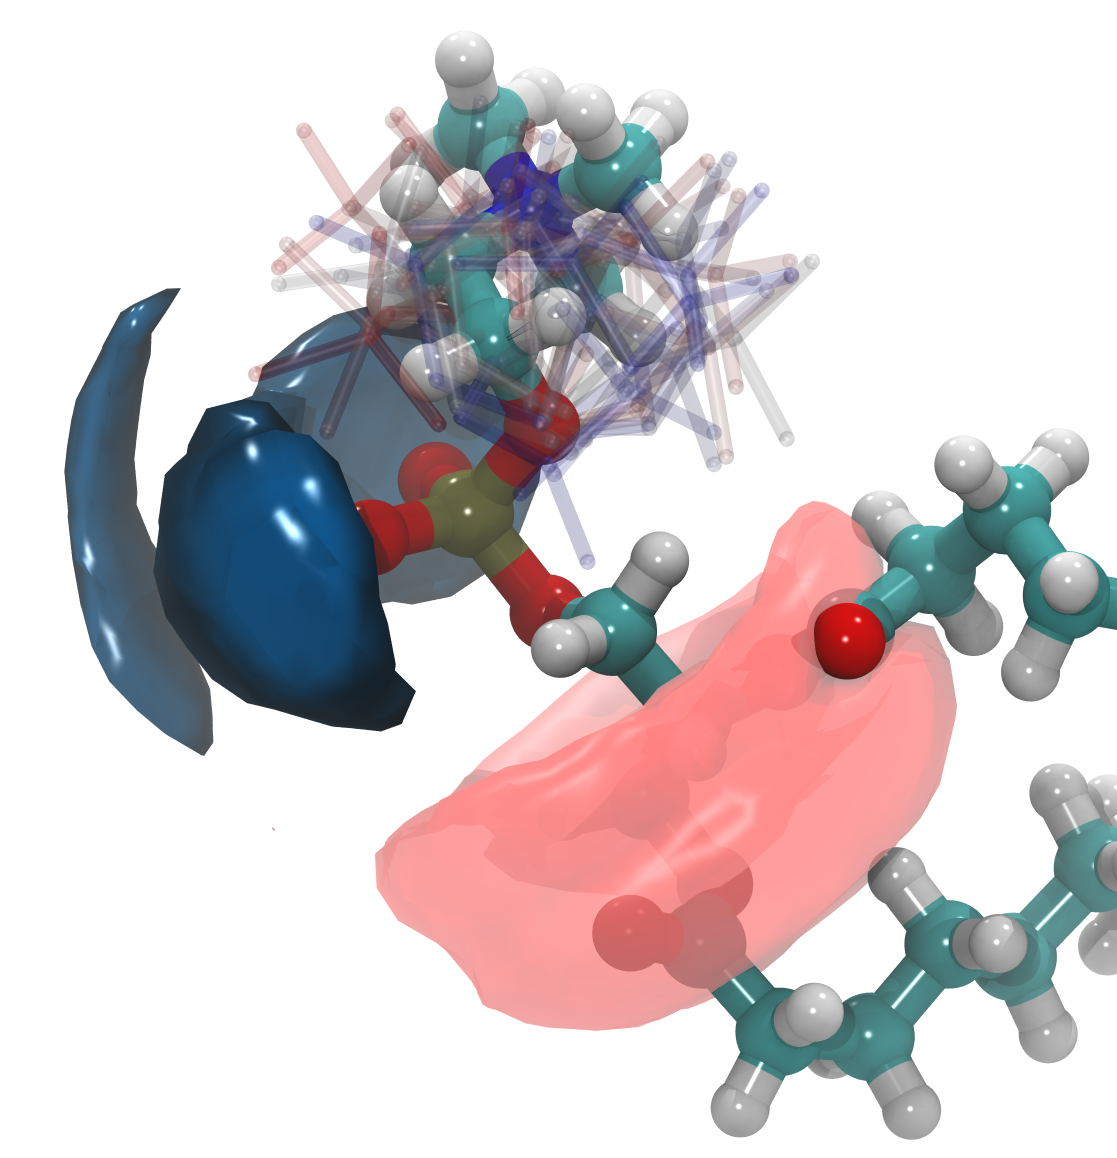
\includegraphics[width=8.0cm]{../img/ecc_pops/isocontours_r37_ca_O-carb.png} 
  \caption{\label{fig:volmaps} 
    Isocontours of spatial number density of \ce{Ca^{2+}} (dark blue, 0.001~Å$^{-3}$) 
    and POPC carbonyl oxygen atoms (light semi-transparent red, 0.008~Å$^{-3}$, all POPC lipids contribute). 
    Calcium cations localize mostly around phosphate oxygens (oxygens red, phosphorus bronze).
    Interactions with carbonyl oxygens is less likely than with phosphate oxygens, 
    and it is contributed more by other neighbouring phospholipids than by the same lipid. 
    Transparent structures are shown to depict the variability of choline configurations 
    (colour warps from red to blue along the simulation time). 
    The number density was evaluated for each lipid, 
    after its structural alignment using only phosphate group.
    MDAnalysis \cite{mdanalysis2011} library was used for 
    the calculations of the structural alignment and the spatial number density. 
    VMD \cite{hump96} was used for visualisation. 
    Carbon atoms are depicted in cyan, hydrogen atoms in white, oxygen atoms in red, nitrogen in blue.
  } 
\end{figure} 
 
Even though \ce{Na+} ions do not bind strongly to a POPC bilayer, they still interact mostly with its oxygen moieties. The results from a simulation at a $1\,$M \ce{NaCl} concentration show that 55\% of \ce{Na+} ions at the bilayer interact with phosphate oxygens of POPC only and 20\% with carbonyl oxygens only, with the remaining 25\%, is interacting with both negatively charged groups. 
 
In conclusion, the results suggest that calcium ions bind specifically to the phosphate oxygens, occasionally interacting also with the carbonyls of the PC lipids. This is in a qualitative agreement with previous conclusions from several experimental studies~\cite{hauser76, hauser78, herbette84, cevc90, binder02}. However, the present results suggest, in 
agreement with experiments, an overally weaker binding to the bilayer, in particular with a lower relative binding affinity to the carbonyls than inferred from previous MD simulation studies~\cite{bockmann03, bockmann04, melcrova16, javanainen17}. Sodium ions, which do not exhibit any appreciable affinity for the bilayer, also interact primarily with phosphate oxygens of the POPC, but in contrast to calcium, the interactions purely with carbonyls are also significant. 
 
 
\subsection{Binding stoichiometry of \ce{Na+} and \ce{Ca^{2+}} cations to POPC membrane} 
Simple binding models have been used previously to interpret the same experimental data \cite{altenbach84,macdonald87} as employed in this work to validate the simulation models (Fig.~\ref{fig:delta_ordPar_CaCl}). In particular, NMR data concerning the PC headgroup order parameters response and atomic absorption spectra were explained best using a ternary complex binding model with a binding stoichiometry of one \ce{Ca^{2+}} per two POPC lipids~\cite{altenbach84}. Nevertheless, a Langmuir adsorption model assuming a \ce{Ca^{2+}}:POPC stoichiometry of 1:1 also provided a good fit to the experimental data when considering \ce{CaCl2} at low concentrations only~\cite{macdonald87}. 
 
 
In this work, we reproduce the same experimental data used to infer binding stoichiometries employing our ECC-POPC model. Thanks to our simulations, we have a direct access to atomistic details of the binding stoichiometry without a need for any binding model as employed for interpreting in experiments~\cite{altenbach84, macdonald87}.
To evaluate the relative propensities for each of the stoichiometric complexes (i.e.,~1~Ca$^{2+}$:~n~POPC),
we calculated for each bound Ca$^{2+}$ the number of POPC molecules having oxygen atoms within a distance of 0.3~nm.
Results from the POPC bilayer simulation with a 285~mM bulk concentration of CaCl$_2$ are shown in Fig.~\ref{fig:cacl_complexes}. 
We found the largest propensity for the 1:2 complex (41\%), with probabilities of complexes with the stoichiometries of 1:1~(25\%)~and 1:3~(34\%)~being only slightly lower. This suggests a more complex binding model than considered in a simple 1:2 ternary complex model previously. Nevertheless, with a broad brushstroke, the simulation data can be viewed such that one calcium binds to two lipids on average, because the probabilities of the complexes with 1 or 3 lipids are almost equal to each other  (and complexes with more than three lipids per one calcium ion were not observed). This probably explains why the simple the ternary complex model fits adequately the experimental data, as well as the ECC-POPC simulation results (see Fig.~S3 in SI). 
 
\begin{figure}[tb!] 
  \centering 
  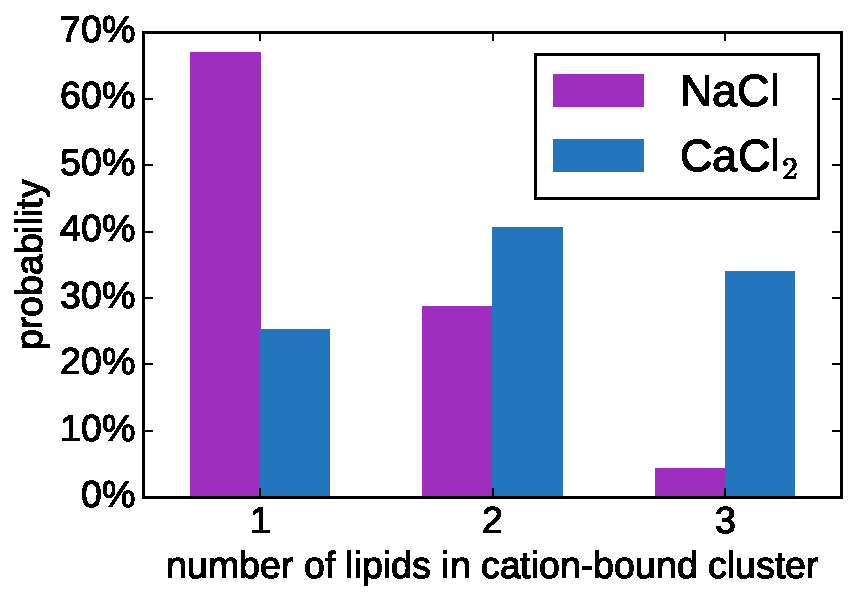
\includegraphics[width=8.0cm]{../img/ecc_pops/stoichiometry_NaCl-CaCl2_comparison_Ecc-lipids.pdf} \\ 
  \caption{\label{fig:cacl_complexes} 
      Relative probabilities of existence of \ce{Na^{+}} or \ce{Ca^{2+}} complexes 
      with a certain number of POPC lipids.  
      \ce{Na^{+}} complexes were evaluated from the simulation with 1~M concentration; 
      and \ce{Ca^{2+}} complexes were evaluated from the simulation with 287~mM concentration. 
  } 
\end{figure} 
 
The probabilities of different complexes formed by \ce{Na+} ions and POPC 
analyzed from the simulation with the ECC-POPC model at $1\,$M concentration of NaCl are also  
shown in Fig.~\ref{fig:cacl_complexes}. In contrast to calcium, the 
probability is largest (67\%) for 1:1 complex, significantly smaller (29\%) 
for 1:2 complexes and very small (4\%) for 1:3 of \ce{Na+}:POPC complexes. 
 
 
 
 
\subsection{Residence times of \ce{Na+} and \ce{Ca^{2+}} cations in the POPC membrane} 
 
Equilibration of \ce{Ca^{2+}} ions at a POPC bilayer in MD simulations is a microsecond time scale process with current force fields, such  as CHARMM36 and Slipids force fields~\cite{javanainen17}. This suggests that at least several microseconds are required to reach the ion binding/unbinding equilibrium. 
To quantify the exchange of ions between the membrane and aqueous solution in simulations, we evaluated residence times of ions bound to the membrane. Within our analysis, an ion is considered to be bound when it is within 0.3~nm from any oxygen atom belonging to a POPC molecule. 
 
The histograms of residence times of \ce{Ca^{2+}} in a POPC bilayer ($C_{ion}'$ = 450~mM) from simulations with  
ECC-POPC and CHARMM36 (simulation from Refs.~\citenum{javanainen17,zenodo.259376}) are shown in Fig.~S4 in SI. 
In the CHARMM36 simulation, a significant number of the calcium ions is bound to the membrane for the whole length of the trajectory (800~ns). 
In contrast, at least an order of magnitude faster bound/unbound calcium exchange is observed within the ECC-POPC model, 
where 90\% of the \ce{Ca^{2+}} residence times to a POPC membrane are shorter than $60\,\mathrm{ns}$. The longest observed 
residence time is around 150~ns, which is below the total length of the simulation used for analysis, i.e., 200~ns. 
Note that these results are in line with the experimental estimate that the residence time of \ce{Ca^{2+}} at each PC 
headgroup is of the order of $10\,\mu\mathrm{s}$~\cite{altenbach84}. Note that the exchange of \ce{Na+} ions at the POPC membrane 
is yet another order of magnitude faster, with 90\% of the residence times smaller than~1~ns and the longest residence time being~6~ns. 
 
In summary, the results from the ECC-POPC model suggest that the exchange of calcium between the POPC bilayer and the solvent occurs within the $\sim$100~ns timeframe, which is significantly faster than observed in simulations emloying most of the presently available lipid models~\cite{javanainen17}. Sodium cations exhibit an even more rapid exchange between the membrane and the aqueous solution. Our results suggest that simulations with a length of several hundreds of nanoseconds are sufficient to simulate alkali and alkali earth ion binding to phospholipid bilayers in equilibrium when realistic force fields are used. This has not been the case with previous lipid force fields, which overestimate the binding strength of the sodium and, in particular,  calcium cations \cite{javanainen17, catte16}. 
 
 
